\subsection{Galerkin}
\begin{frame}
	\only<1->{
	\begin{block}{Ecuacion de Burgers' Determinista}
		\begin{equation*}
		\frac{\partial u(x, t)}{\partial t} +  \frac{1}{2} \frac{\partial \left[ u(x, t) \right]^2}{\partial x} - \alpha \frac{\partial^2 u(x, t)}{\partial x^2} = 0.
		\end{equation*}
	\end{block}
	}
	\only<2->{
	Usando el operador proyecci\'on
	\begin{equation*}
	u_N (x, t) = \displaystyle \sum_{ |n| \leq \frac{N}{2} } \hat{u}_n e^{inx} 
	\end{equation*}
	}
	\only<3->{
	\begin{block}{Aproximacion por Fourier-Galerkin}
		\begin{equation*}
		\left \lbrace \begin{array}{ll}
		u_N(t): [0, T] \rightarrow V_N, \hspace{2mm} \text{t.q para cada} \hspace{2mm} \phi \in V_N \\
		\\
		( \frac{\partial u_N}{\partial t} + \frac{1}{2} (u_N^2)_x -  \alpha \frac{\partial^2 u_N}{\partial x^2}, \phi) = 0 \\
		\\
		u_N(0) = \mathcal{P}_N u_0 (x)
		\end{array}  \right .
		\end{equation*}
	\end{block}
	}
\end{frame}

\begin{frame}
	\only<1->{
	\begin{equation*}
	\displaystyle \frac{1}{2\pi} \int_{0}^{2 \pi} \left( \frac{\partial u_{N}}{\partial t} + \frac{1}{2} \frac{\partial}{\partial x} \left( u^2_N \right) - \alpha \frac{\partial^2 u_N}{\partial x^2} \right) e^{inx} dx = 0, \hspace{0.3cm} \forall |n| \leq \frac{N}{2} 
	\end{equation*}
	}
	\only<2->{
	\begin{equation*}
	\frac{d \hat{u}_n (t)}{dt} = \alpha p^2 n^2 \hat{u}_n (t) - p \widehat{G}_n (t) , \hspace{0.3cm} \forall |n| \leq \frac{N}{2} 
	\end{equation*}
	}
	\only<3->{
	Discretizando la variable temporal $t$ en el intervalo $[0, T]$ 
	\begin{equation*}
	t_j = j \Delta t, \hspace{2mm} j = 0, 1, \dots, T.
	\end{equation*} 
	}
	\only<4->{
	y para la variable espacial $x$ en el intervalo $[x_L, x_R]$, definiendo $x_n = p z_n + x_L$, $p = \frac{x_R - x_L}{2 \pi}$,  
	\begin{equation*}
	z_n = \frac{2 \pi n}{N}, \hspace{2mm} n = 0, 1, \dots, N.
	\end{equation*}
	}
\end{frame}

\begin{frame}
	\begin{block}{Discretizaci\'on Semi-Impl\'icita}
	\begin{equation*}
	\hat{u}_n (t_{j+1}) = \hat{u}_n (t_j) + \Delta t \left[\alpha p^2 n^2 \hat{u}_n (t_j) - p \widehat{G}_n (t_{j+1})  \right],
	\end{equation*}
	Donde $\widehat {G}_n $ 
	\begin{equation*}
	\widehat{G}_n (t_{j+1}) = \displaystyle in \left[ \sum_{|k| \leq \frac {N}{2}} \hat{u}_n (t_{j+1}) \hat{u}_{n - k} (t_{j+1}) \right].
	\end{equation*}
	\end{block}
\end{frame}

\begin{frame}
	\only<1->{	
	Finalmente es evaluada la solucion numerica
	\begin{equation*}
	u_N(x, t_j) = \displaystyle \sum_{|n| \leq \frac{N}{2}} \hat{u}_n (t_j) e^{inx}
	\end{equation*}
	}
	\only<2->{
	Para los siguientes resultados numericos se considero lo siguiente	
	\begin{equation*}
		u_0 (x) = e^{-0.05 x^2}, \hspace{3mm} x \in [-60, 60], \hspace{2mm} t \in [0, 100]. 
	\end{equation*}
	}
\end{frame}

\begin{frame}	
	\centering
	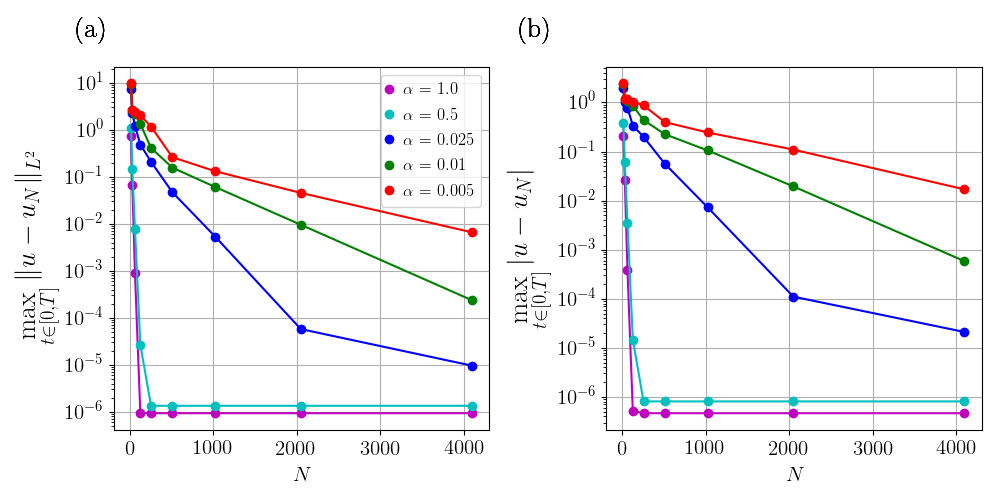
\includegraphics[width=11cm]{FIGURES/Galerkin/Graphics/alphas_Error_N.png}
	$N = 2^m$, $m = 4, \dots, 12$; $\Delta t = 1.0 \times 10^{-5}$.
\end{frame}
\begin{frame}	
	$\alpha = 1.0$; $N=2048$; $\Delta t = 1.0 \times 10^{-5}$.
	\centering
	\includegraphics[width=7.5cm]{FIGURES/Galerkin/Graphics/eps=1.0/Numerical_Solution_alpha=1.png}
\end{frame}
\begin{frame}
	$t = 100$, $\alpha = 1.0$, $\Delta t = 1.0 \times 10^{-5}$.
	\centering
	\includegraphics[width=10cm]{FIGURES/Galerkin/Graphics/eps=1.0/Numerical_Solution_alpha=1_T=100.png}
\end{frame}

\begin{frame}
\begin{table}
	\centering
	\begin{tabular}{lcccc}
		\toprule
		\multicolumn{1}{c}{\textbf{Approximation}} & \multicolumn{4}{c}{\textbf{Error}} \\
		$\hspace{9mm}N$ & $\Delta t=1\times 10^{-2}$ & $\Delta t=1\times 10^{-3}$ & $\Delta t=1\times 10^{-4}$ & $\Delta t=1\times 10^{-5}$ \\
		\midrule
		\hspace{7mm} 16 & 0.72504    & 0.72504    & 0.72504    & 0.72504    \\
		\midrule
		\hspace{7mm} 32 & 6.90249 $\times 10 ^{-2}$   & 6.88052 $\times 10 ^{-2}$   & 6.87838 $\times 10 ^{-2}$   & 6.87816 $\times 10 ^{-2}$   \\
		\midrule
		\hspace{7mm} 64 & 1.23827 $\times 10 ^{-3}$  & 8.85367 $\times 10 ^{-4}$ & 8.80521 $\times 10 ^{-4}$ & 8.80410 $\times 10 ^{-4}$  \\
		\midrule
		\hspace{7mm} 128 & 9.43454 $\times 10 ^{-4}$ & 9.41793 $\times 10 ^{-5}$ & 9.41148 $\times 10 ^{-6}$ & 9.41827 $\times 10 ^{-7}$  \\
		\midrule
		\hspace{7mm} 256 & 9.43454 $\times 10 ^{-4}$ & 9.41793 $\times 10 ^{-5}$ & 9.41109 $\times 10 ^{-6}$ & 9.36411 $\times 10 ^{-7}$ \\
		\midrule
		\hspace{7mm} 512 & 9.43454 $\times 10 ^{-4}$ & 9.41793 $\times 10 ^{-5}$ & 9.41109 $\times 10 ^{-6}$ & 9.36411 $\times 10 ^{-7}$ \\
		\midrule
		\hspace{7mm} 1024 & $\ast$ & 9.41793 $\times 10^{-5}$ & 9.41109 $\times 10^{-6}$ & 9.36411 $\times 10^{-7}$              \\
		\midrule
		\hspace{7mm} 2048 & $\ast$ & $\ast$ & 9.41109 $\times 10^{-6}$ & 9.36411 $\times 10^{-7}$   \\
		\\
		\bottomrule
	\end{tabular}
\end{table}
\end{frame}

\begin{frame}
	$\alpha = 0.005$; $N=2048$; $\Delta t = 1.0 \times 10^{-5}$.
	\centering
	\includegraphics[width=7.5cm]{FIGURES/Galerkin/Graphics/eps=0.005/Numerical_Solution_alpha=0005.png}
\end{frame}
\begin{frame}
	$t = 100$; $\alpha = 0.005$; $\Delta t = 1.0 \times 10^{-5}$.
	\centering
	\includegraphics[width=10cm]{FIGURES/Galerkin/Graphics/eps=0.005/Numerical_Solution_alpha=0005_T=100.png}
\end{frame}

\begin{frame}
\begin{table}
	\begin{tabular}{lcccc}
		\toprule
		\multicolumn{1}{c}{\textbf{Approximation}} & \multicolumn{4}{c}{\textbf{Error}} \\
		$\hspace{9mm}N$ & $\Delta t=1\times 10^{-2}$ & $\Delta t=1\times 10^{-3}$ & $\Delta t=1\times 10^{-4}$ & $\Delta t=1\times 10^{-5}$ \\
		\midrule
		\hspace{7mm} 16 & 9.95328   & 9.91901    & 9.91597    & 9.91567    \\
		\midrule
		\hspace{7mm} 32 & 2.72607   & 2.70558    & 2.70347    & 2.70326    \\
		\midrule
		\hspace{7mm} 64 & 2.50343   & 2.45988    & 2.45543    & 2.45497    \\
		\midrule
		\hspace{7mm} 128 & 2.16142   & 2.06992    & 2.05918    & 2.05795    \\
		\midrule
		\hspace{7mm} 256 & 1.3658    & 1.19385    & 1.17602    & 1.17412    \\
		\midrule
		\hspace{7mm} 512 & 0.339826  & 0.265843   & 0.262164   & 0.261805   \\
		\midrule
		\hspace{7mm} 1024 & 0.161405  & 0.133743   & 0.131882   & 0.131699   \\
		\midrule
		\hspace{7mm} 2048 & 6.50292 $\times 10^{-2}$ & 4.70602 $\times 10^{-2}$ & 4.57371 $\times 10^{-2}$  & 4.56090 $\times 10^{-2}$  \\
		\midrule
		\hspace{7mm} 4096 & * & 7.26917 $\times 10^{-3}$ & 6.64157 $\times 10^{-3}$ & 6.60753 $\times 10^{-3}$ \\
		\\
		\bottomrule
	\end{tabular}
\end{table}
\end{frame}

\subsection{Colocacion}
\begin{frame}
	\only<1->{
	\begin{block}{Aproximacion por Fourier-Colocaci\'on}	
	\begin{equation*}
		\left \lbrace \begin{array}{ll}
		u_N(t): [0, T] \rightarrow V_N, \hspace{2mm} \text{t.q para cada} \hspace{2mm} \phi \in V_N  \\
		\\
		\left\langle \frac{\partial u_N}{\partial t}, \phi \right\rangle_N - \left\langle \frac{\partial^2 u_N}{\partial x^2}, \phi \right\rangle_N + \frac{1}{2} \left\langle \mathcal{J}_N (u_N^2)_x, \phi \right\rangle_N = 0, \hspace{2mm} t > 0, \hspace{2mm} x \in I \\
		\\
		u_N(0) = \mathcal{J}_N u_0 (x), \hspace{2mm} t = 0, \hspace{2mm} x \in I
		\end{array}  \right .
	\end{equation*}	
	\end{block}
	}
	\only<2->{
	\begin{equation*}
		u_N (x, t) =  \displaystyle \sum_{|n| \leq \frac {N}{2}} \widetilde{u}_n (t) e^{inx}, \hspace{2mm} x_j = \frac{2 \pi j}{N + 1}, \hspace{2mm} j\in [0, \dots , N]. 
	\end{equation*}
	}
	\begin{equation*}
	R_{N} (x_j, t) = \frac{\partial u_N}{\partial t} (x_j, t) - \frac{\partial^2 u_N }{\partial x^2} (x_j, t) + \frac{1}{2} \mathcal{J}_N \left(u^2_N \right)_x (x_j, t) = 0
	\end{equation*}
\end{frame}

\begin{frame}	
	\only<1->{
	Necesitamos resolver las $N + 1$ ecuaciones diferenciales con condiciones iniciales $u_N (x_j, 0) = u_0(x_j)$, pero primeramente hacemos la siguiente notacion:
	\begin{equation*}
		u_N (t) = (u_N (x_0 , t), u_N (x_1 , t), \dots , u_N (x_{N} , t))^T,
	\end{equation*} 
	
	\begin{equation*}
	\frac{d u_N (t)}{dt} + \frac{1}{2} D_N u^2_N (t) - D_N^2 u_N (t) = 0,
	\end{equation*}
	}
	\only<2->{
	\begin{block}{Discretizacion Semi-Implicita}	
	\begin{equation*}
		u_N (t_{i + 1} ) = u_N (t_i) + \Delta t \left[p^2 D_N^2 u_N (t_i) - \frac{1}{2} p D_N u^2_N (t_{i+1}) \right].
	\end{equation*}
	\end{block}
	}
\end{frame}

\begin{frame}
	\only<1->{
	Discretizacion de $t$ en $[0, T]$
	\begin{equation*}
		t_i = i \Delta t, \hspace{2mm} i = 0, 1, \dots, T,
	\end{equation*} 
	}
	\only<2->{
	Discretizacion espacial $x$ en $[x_L, x_R]$, $x_j = p z_j + x_L$, $p = \frac{x_R - x_L}{2 \pi}$
	\begin{equation*}
		z_j = \frac{2 \pi j}{2N + 1}, \hspace{2mm} n = 0, 1, \dots, N.
	\end{equation*}
	}
	\only<3->{
	Finalmente, evaluamos la solucion numerica
	\begin{equation*}
		u_N(x, t_i) = \displaystyle \sum_{|n| \leq N} \hat{u}_n (t_i) e^{inx}
	\end{equation*}
	}
	\only<4->{
	Como anteriormente, se considero lo siguiente para los siguientes resultados numericos
	\begin{equation*}
		u_0 (x) = e^{-0.05 x^2}, \hspace{3mm} x \in [-60, 60], \hspace{2mm} t \in [0, 100]. 
	\end{equation*}
	}
\end{frame}

\begin{frame}
	$N = 2^m$, $m = 4, \dots, 11$; $\Delta t = 1.0 \times 10^{-5}$.
	\centering
	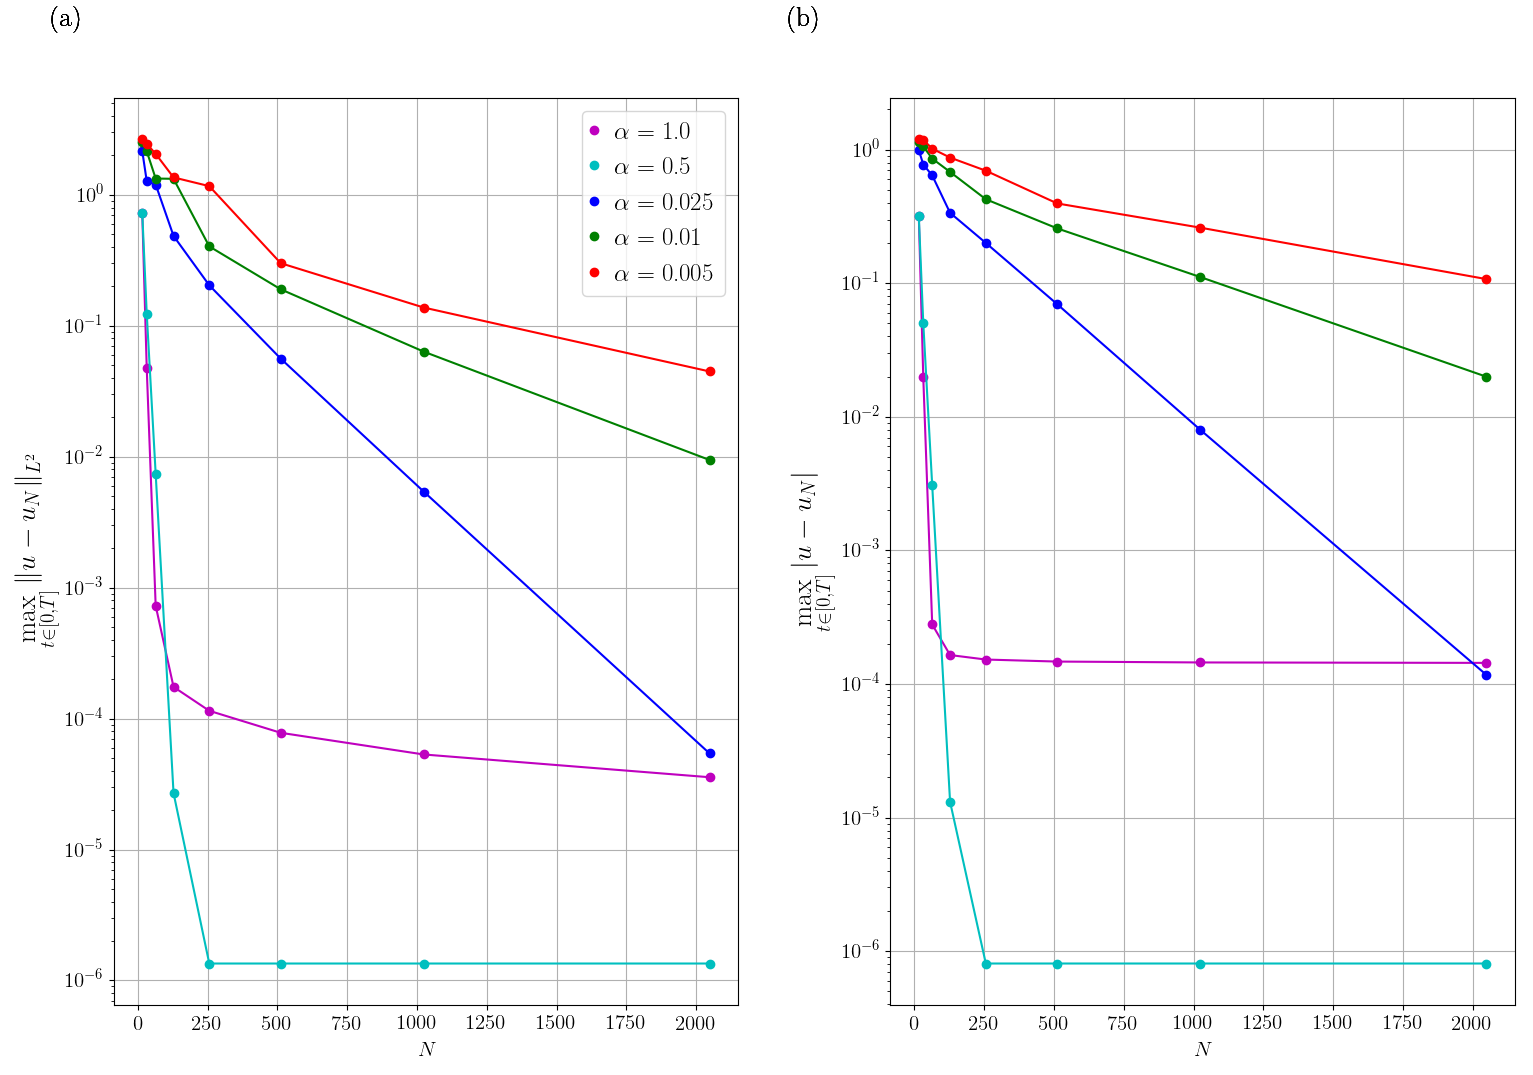
\includegraphics[width=9cm]{FIGURES/Collocation/collocation_alphas_N.png}
\end{frame}	

\begin{frame}
	$\alpha = 1.0$; $N=2048$; $\Delta t = 1.0 \times 10^{-5}$.
	\centering
	\includegraphics[width=7.5cm]{FIGURES/Collocation/Graphics/eps=1.0/Numerical_Solution_alpha=1.png}
\end{frame}
\begin{frame}
	$t = 100$, $\alpha = 1.0$, $\Delta t = 1.0 \times 10^{-5}$.
	\centering
	\includegraphics[width=10cm]{FIGURES/Collocation/Graphics/eps=1.0/Numerical_Solution_alpha=1_T=100.png}
\end{frame}

\begin{frame}
\begin{table}
	\begin{tabular}{lcccc}
		\toprule
		\multicolumn{1}{c}{\textbf{Approximation}} & \multicolumn{4}{c}{\textbf{Error}} \\
		$\hspace{9mm}N$ & $\Delta t=1\times 10^{-2}$ & $\Delta t=1\times 10^{-3}$ & $\Delta t=1\times 10^{-4}$ & $\Delta t=1\times 10^{-5}$ \\
		\midrule
		\hspace{7mm} 16 & 0.721112    & 0.721112    & 0.721112    & 0.721112    \\
		\midrule
		\hspace{7mm} 32 & 4.71797 $\times 10^{-2}$   & 4.72892 $\times 10^{-2}$   & 4.73004 $\times 10^{-2}$   & 4.73015 $\times 10^{-2}$   \\
		\midrule
		\hspace{7mm} 64 & 1.17954 $\times 10^{-3}$  & 7.35344 $\times 10^{-4}$ & 7.27561 $\times 10^{-4}$ & 7.27283 $\times 10^{-4}$  \\
		\midrule
		\hspace{7mm} 128 & 9.43454 $\times 10^{-4}$ & 1.75152 $\times 10^{-4}$ & 1.74583 $\times 10^{-4}$ & 1.74574 $\times 10^{-4}$ \\
		\midrule
		\hspace{7mm} 256 & 9.43454 $\times 10^{-4}$ & 1.15509 $\times 10^{-4}$ & 1.14669 $\times 10^{-4}$ & 1.14659 $\times 10^{-4}$ \\
		\midrule
		\hspace{7mm} 512 & 9.43454 $\times 10^{-4}$ & 9.41793 $\times 10^{-5}$ & 7.78847 $\times 10^{-5}$ & 7.78707 $\times 10^{-5}$ \\
		\midrule
		\hspace{7mm} 1024 & 0           & 9.41793 $\times 10^{-5}$ & 5.32213 $\times 10^{-5}$ & 5.32019 $\times 10^{-5}$ \\
		\midrule
		\hspace{7mm} 2048 & 0           & 0           & 3.56779 $\times 10^{-5}$ & 3.56498 $\times 10^{-5}$ \\
		\midrule
		\hspace{7mm} 4096 & 0           & 0           & 2.24122 $\times 10^{-5}$ & 0           \\
		\\
		\bottomrule
	\end{tabular}
\end{table}
\end{frame}

\begin{frame}
	$\alpha = 0.005$; $N=2048$; $\Delta t = 1.0 \times 10^{-5}$.
	\centering
	\includegraphics[width=7.5cm]{FIGURES/Collocation/Graphics/eps=0.005/Numerical_Solution_alpha=0005.png}
\end{frame}	
\begin{frame}
	$t = 100$, $\alpha = 1.0$, $\Delta t = 1.0 \times 10^{-5}$.
	\centering
	\includegraphics[width=10cm]{FIGURES/Collocation/Graphics/eps=0.005/Numerical_Solution_alpha=0005_T=100.png}
\end{frame}

\begin{frame}
\begin{table}
	\begin{tabular}{lcccc}
		\toprule
		\multicolumn{1}{c}{\textbf{Approximation}} & \multicolumn{4}{c}{\textbf{Error}} \\
		$\hspace{9mm}N$ & $\Delta t=1\times 10^{-2}$ & $\Delta t=1\times 10^{-3}$ & $\Delta t=1\times 10^{-4}$ & $\Delta t=1\times 10^{-5}$ \\
		\midrule
		\hspace{7mm} 16 & 1.36189   & 1.35883    & 1.35852   & 1.35849   \\
		\midrule
		\hspace{7mm} 32 & 2.67506   & 2.65305    & 2.65078   & 2.65055   \\
		\midrule
		\hspace{7mm} 64 & 2.50365   & 2.45855    & 2.45432   & 2.45387   \\
		\midrule
		\hspace{7mm} 128 & 2.15795   & 2.0632     & 2.05589   & 2.05497   \\
		\midrule
		\hspace{7mm} 256 & 1.362     & 1.18393    & 1.16697   & 1.16532   \\
		\midrule
		\hspace{7mm} 512 & 0.350775  & 0.304595   & 0.300865  & 0.300499  \\
		\midrule
		\hspace{7mm} 1024 & 0.168462  & 0.140332   & 0.13803   & 0.137804  \\
		\midrule
		\hspace{7mm} 2048 & 6.56161 $\times 10^{-2}$ & 4.63808 $\times 10^{-2}$  & 4.49226 $\times 10^{-2}$ & 4.47813 $\times 10^{-2}$ \\
		\midrule
		\hspace{7mm} 4096 & 0         & 7.66246 $\times 10^{-3}$ & 6.9909 $\times 10^{-3}$ & 0         \\
		\\
		\bottomrule
	\end{tabular}
\end{table}
\end{frame}

\subsection{Bajos Coeficientes de Viscosidad}
\begin{frame}
	\frametitle{Bajos Coeficientes de Viscosidad}
	\only<1->{
	Las siguientes soluciones, dadas por mediante Fourier-Galerkin, se considero
	\begin{equation*}
	u_0 (x) = e^{-0.005 x^2}, \hspace{3mm} x \in [-60, 60], \hspace{2mm} t \in [0, T_c], 
	\end{equation*}
	}
	\only<2->{
	donde
	\begin{equation*}
		Tc = \min_{x \in \mathbb{R}} \left[  \frac{-1}{u'_0 (x)} \right],
	\end{equation*}
	}
	\only<3->{
	tiempo donde ocurre una discontinuidad de la ecuacion
	\begin{equation*}
		\frac{\partial u(x, t)}{\partial t} +  \frac{1}{2} \frac{\partial \left[ u(x, t) \right]^2}{\partial x} = 0,
	\end{equation*}
	}
	\only<4->{
	la cual tiene como solucion
	\begin{equation*}
		u(x, t) = u_0 (x_0), \hspace{2mm} x_0 = x - u_0 (x_0) t, 
	\end{equation*}
	}
\end{frame}

\begin{frame}
	$t = T_c$; $N=256$; $\Delta t = 1.0 \times 10^{-3}$.
	\centering
	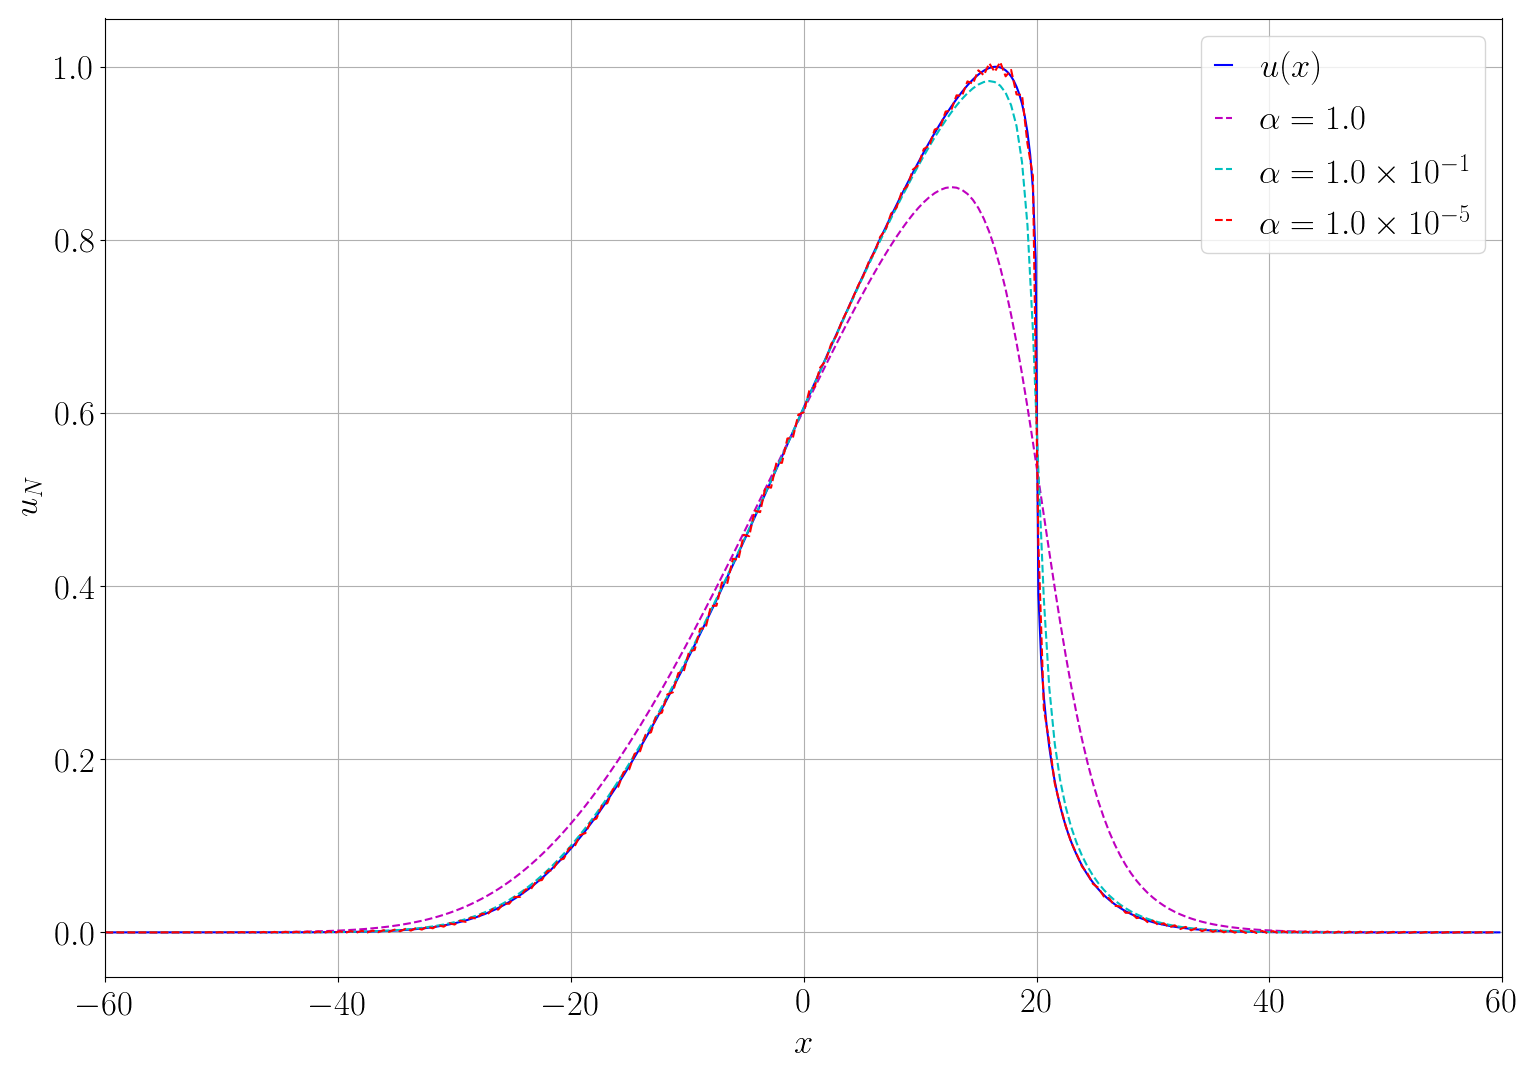
\includegraphics[width=10cm]{FIGURES/varios_alphas.png}
\end{frame}

\begin{frame}
	$\alpha = 1.0 \times 10^{-5}$; $N=256$;  $\Delta t = 1.0 \times 10^{-3}$.
	\centering
	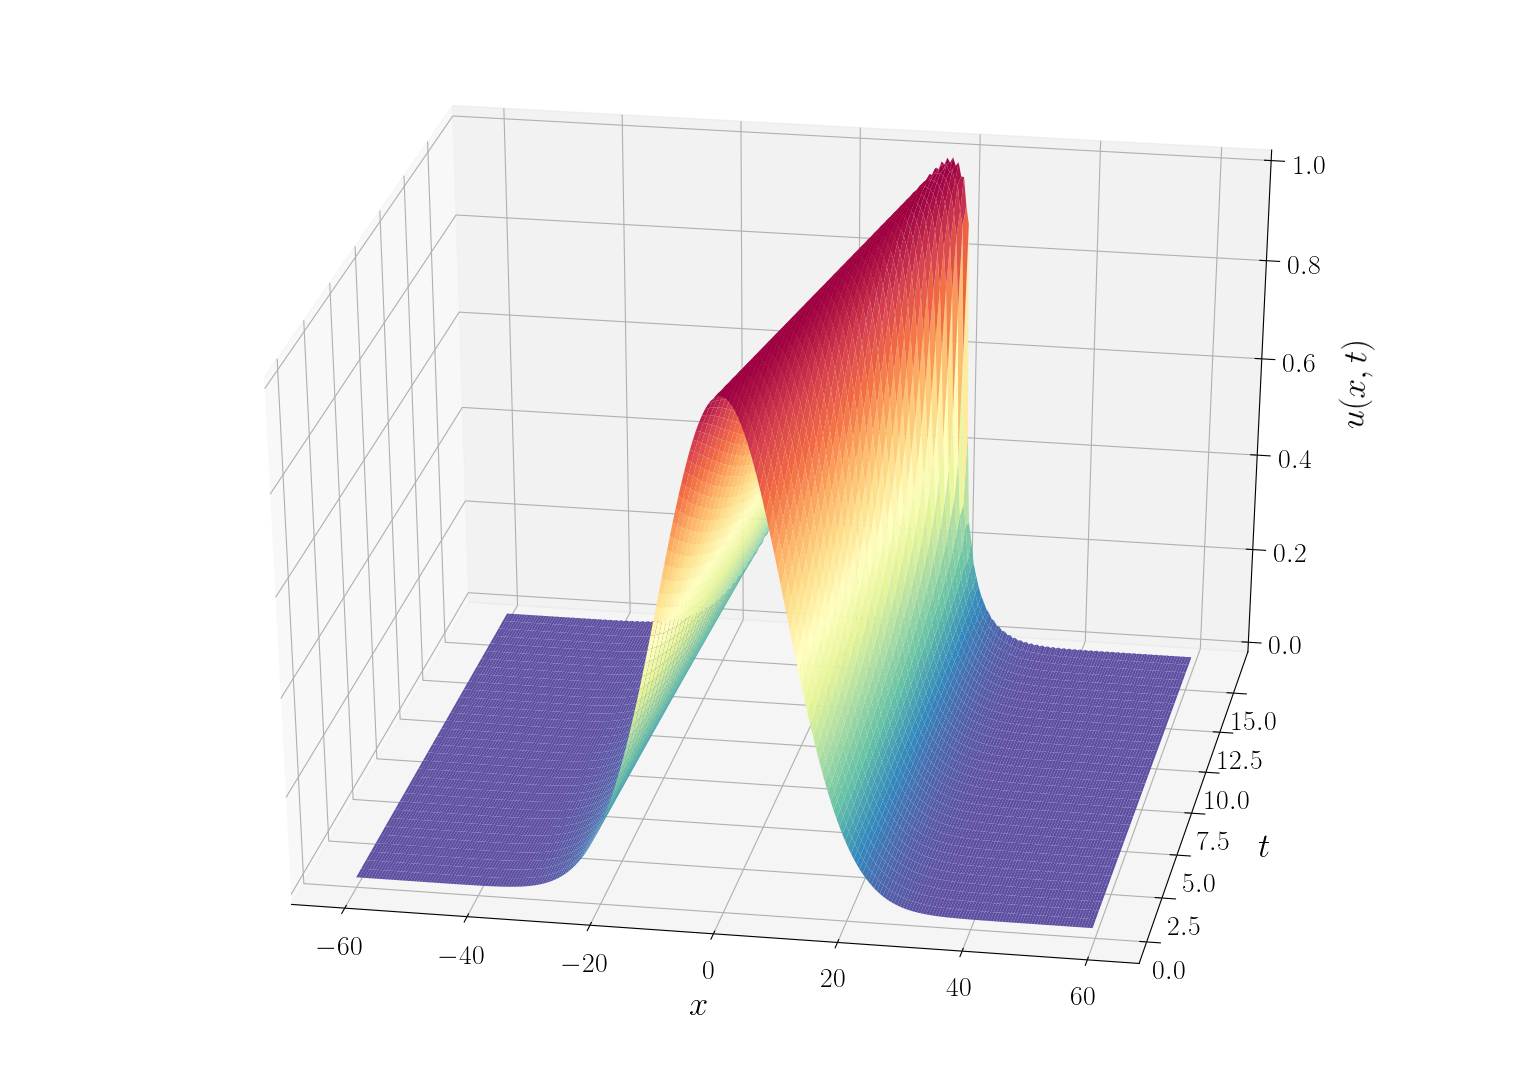
\includegraphics[width=10cm]{FIGURES/small_alpha.png}
\end{frame}

\begin{frame}
	 $t = T_c$; $\alpha = 1.0 \times 10^{-5}$; $\Delta t = 1.0 \times 10^{-3}$.
	\centering
	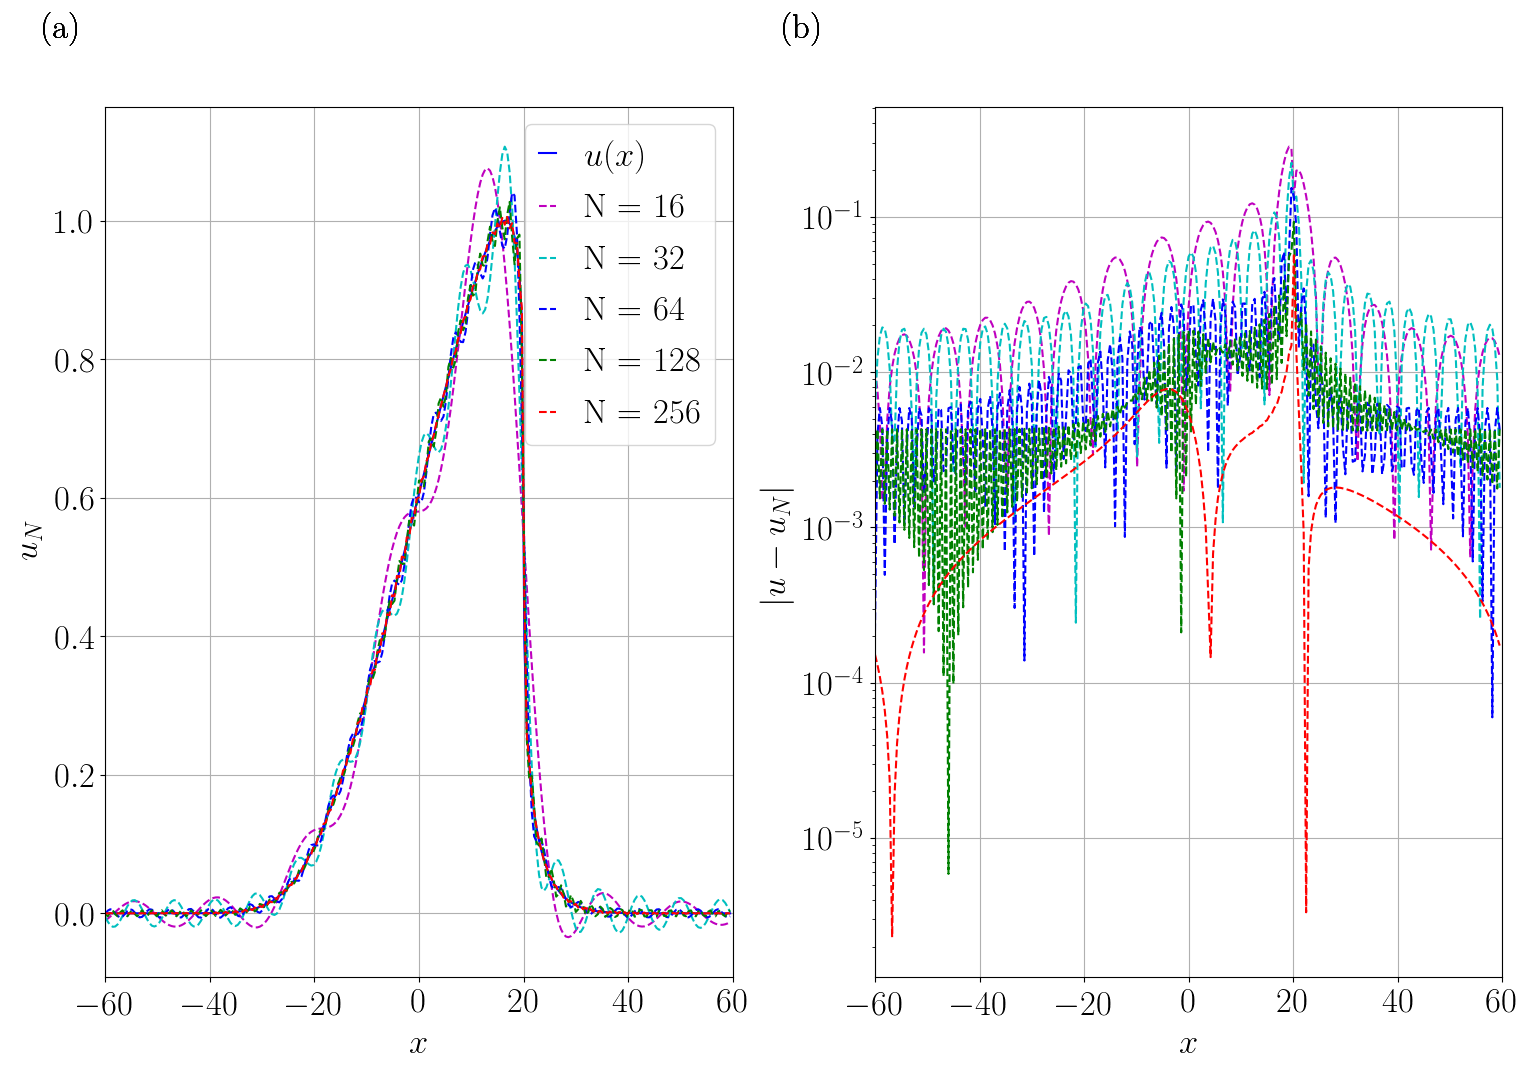
\includegraphics[width=10cm]{FIGURES/small_alpha_T.png}
\end{frame}

\begin{frame}
	\begin{table}
		\centering
		\begin{tabular}{lccc}
			\toprule
			\multicolumn{1}{c}{\textbf{Approximation}} & \multicolumn{3}{c}{\textbf{Distance}} \\
			\hspace{12mm} $N$ & $\Delta t=1\times 10^{-2}$ & $\Delta t=1\times 10^{-3}$ & $\Delta t=1\times 10^{-4}$ \\
			\midrule
			\hspace{12mm} 16 & 0.285531 & 0.285732 & 0.285752 \\
			\midrule
			\hspace{12mm} 32 & 0.222737 & 0.223260 & 0.223312 \\
			\midrule
			\hspace{12mm} 64 & 0.160385 & 0.162782 & 0.163025 \\
			\midrule
			\hspace{12mm} 128 & 0.129297 & 0.133322 & 0.133733 \\
			\midrule
			\hspace{12mm} 256 & 0.083291 & 0.091449 & 0.092320 \\
			\bottomrule
		\end{tabular}
	\end{table}
\end{frame}